\section{Fotometría}

Para este trabajo se realizó una campaña de observación durante los últimos
meses del 2022, con la finalidad de observar el sistema durante una fase orbital
completa. Las fechas y duraciones de cada día de observación se encuentra en la
tabla \ref{observationSchedules}. Durante varias de estas noches de observación
las condiciones del sitio fueron menos que ideal; tanto las condiciones
meteorológicas como contratiempos causados por el equipo en si causaron
interrupciones en la medición del brillo del sistema. Esto es esperado en un
observatorio en proceso de desarrollo; a pesar de los problemas técnicos, se
pudieron obtener datos de calidad aceptable. 

% TODO: style table
\begin{table}[!ht]
	\centering
	\begin{tabular}{|l|l|l|l|}
		\hline
		\thead{Fecha} & \thead{HJD Inicio +\textbf{\num{2459000}}} & \thead{Tiempo Expocisiones} & \thead{Duración} \\
		\hline
		2022-10-21 & 874.6627527894452 & 114 * 60 s & 2.59 h \\
		\hline
		2022-10-27 & 880.7675264584832 & 93 * 60 s & 1.8616666666666666 h \\
		\hline
		2022-11-05 & 889.6711328472011 & 98 * 60 s & 2.0219444444444443 h \\
		\hline
		2022-11-26 & 910.7179540507495 & 56 * 60 s & 1.5502777777777779 h \\
		\hline
		2022-12-06 & 920.5510403933004 & 243 * 60 s & 4.900277777777778 h \\
		\hline
		2022-12-07 & 921.5630493750796 & 163 * 60 s & 4.201388888888889 h \\
		\hline
		2022-12-08 & 922.5338555905037 & 188 * 60 s & 5.570277777777778 h \\
		\hline
		2022-12-09 & 923.5413328357972 & 119 * 60 s & 5.328333333333333 h \\
		\hline
		2022-12-10 & 924.5309011922218 & 122 * 60 s & 2.202777777777778 h \\
		\hline

	\end{tabular}
	\caption{Fechas de observaciones fotométricas desde el OAU.}
	\label{observationSchedules}
\end{table}

\begin{figure}[!ht]
	\centering
	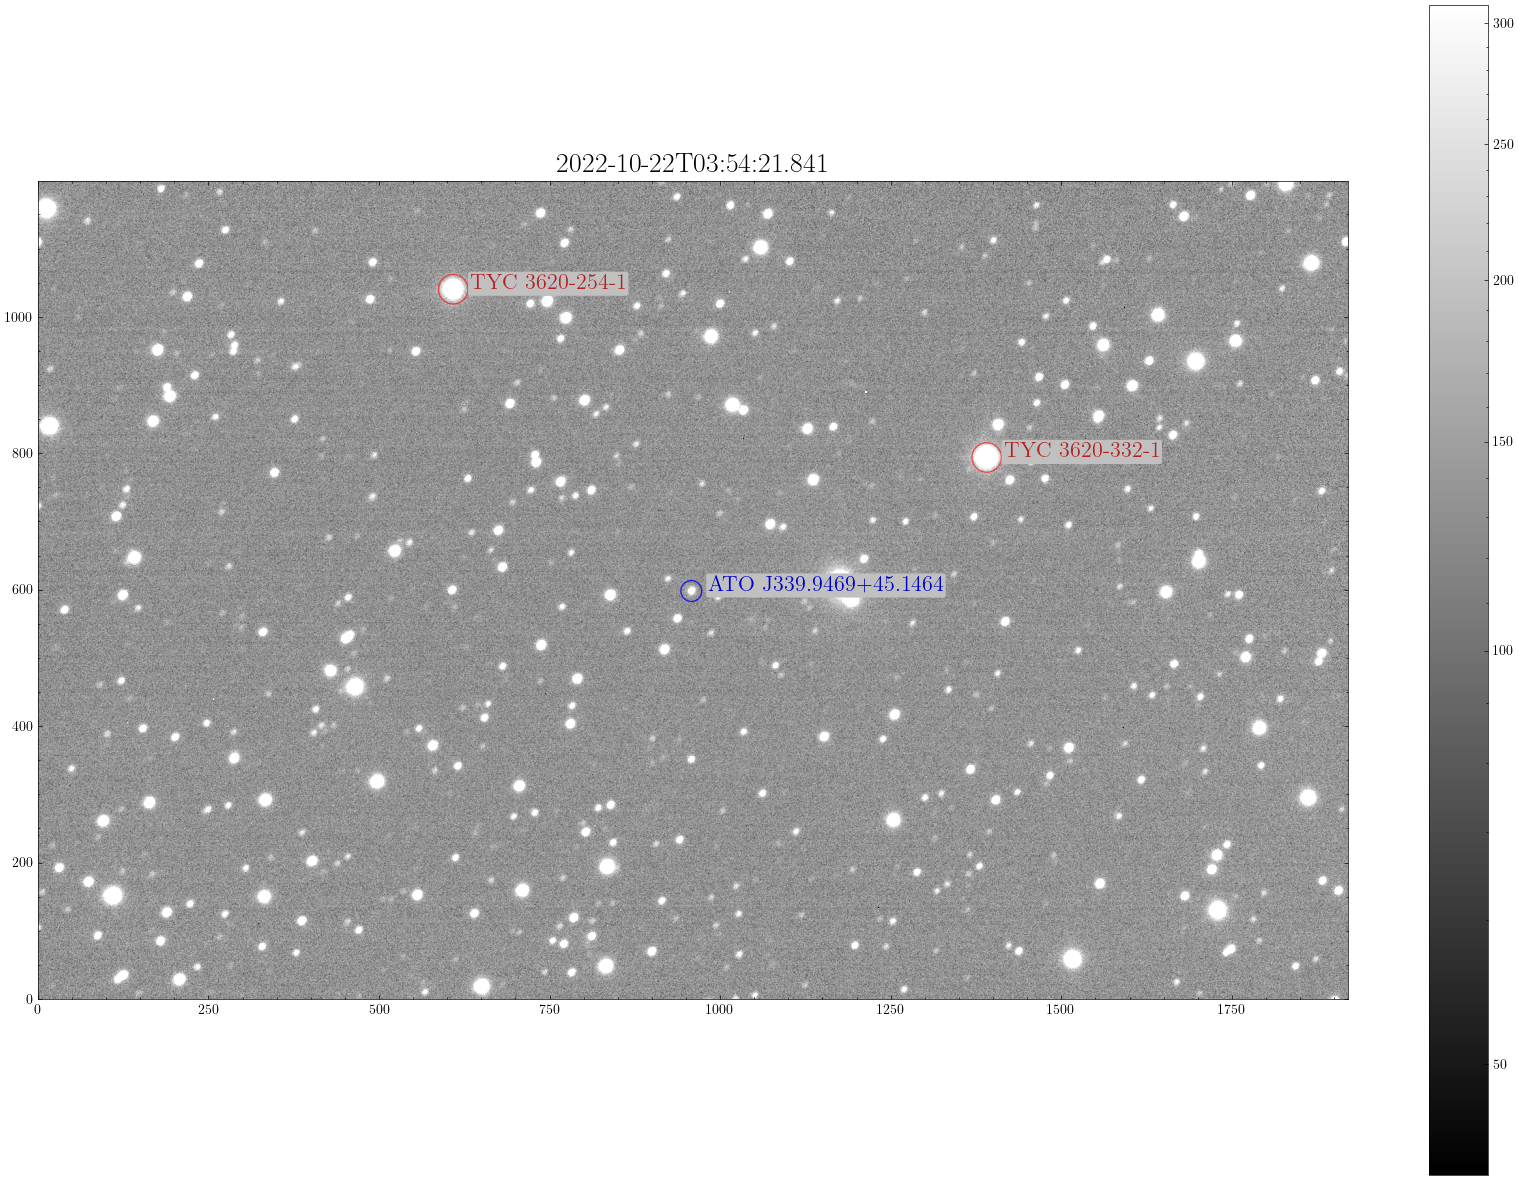
\includegraphics[scale=0.4]{Observaciones/Secciones/Figures/10-22 Sample Image.png}
	\caption{Imagen del campo de \atoObjId, junto a 2 estrellas de comparación usadas en la fotometría diferencial marcadas en anillos rojos.}
	\label{ccdImageField}
\end{figure}

\subsection{Procesamiento de Imágenes}

% TODO: bias, darks, flats
	% scripts from github
	% iraf aperture photometry

\subsection{Fotometría Diferencial}